\documentclass[12pt]{article}\usepackage[]{graphicx}\usepackage[]{color}
%% maxwidth is the original width if it is less than linewidth
%% otherwise use linewidth (to make sure the graphics do not exceed the margin)
\makeatletter
\def\maxwidth{ %
  \ifdim\Gin@nat@width>\linewidth
    \linewidth
  \else
    \Gin@nat@width
  \fi
}
\makeatother

\definecolor{fgcolor}{rgb}{0.345, 0.345, 0.345}
\newcommand{\hlnum}[1]{\textcolor[rgb]{0.686,0.059,0.569}{#1}}%
\newcommand{\hlstr}[1]{\textcolor[rgb]{0.192,0.494,0.8}{#1}}%
\newcommand{\hlcom}[1]{\textcolor[rgb]{0.678,0.584,0.686}{\textit{#1}}}%
\newcommand{\hlopt}[1]{\textcolor[rgb]{0,0,0}{#1}}%
\newcommand{\hlstd}[1]{\textcolor[rgb]{0.345,0.345,0.345}{#1}}%
\newcommand{\hlkwa}[1]{\textcolor[rgb]{0.161,0.373,0.58}{\textbf{#1}}}%
\newcommand{\hlkwb}[1]{\textcolor[rgb]{0.69,0.353,0.396}{#1}}%
\newcommand{\hlkwc}[1]{\textcolor[rgb]{0.333,0.667,0.333}{#1}}%
\newcommand{\hlkwd}[1]{\textcolor[rgb]{0.737,0.353,0.396}{\textbf{#1}}}%

\usepackage{framed}
\makeatletter
\newenvironment{kframe}{%
 \def\at@end@of@kframe{}%
 \ifinner\ifhmode%
  \def\at@end@of@kframe{\end{minipage}}%
  \begin{minipage}{\columnwidth}%
 \fi\fi%
 \def\FrameCommand##1{\hskip\@totalleftmargin \hskip-\fboxsep
 \colorbox{shadecolor}{##1}\hskip-\fboxsep
     % There is no \\@totalrightmargin, so:
     \hskip-\linewidth \hskip-\@totalleftmargin \hskip\columnwidth}%
 \MakeFramed {\advance\hsize-\width
   \@totalleftmargin\z@ \linewidth\hsize
   \@setminipage}}%
 {\par\unskip\endMakeFramed%
 \at@end@of@kframe}
\makeatother

\definecolor{shadecolor}{rgb}{.97, .97, .97}
\definecolor{messagecolor}{rgb}{0, 0, 0}
\definecolor{warningcolor}{rgb}{1, 0, 1}
\definecolor{errorcolor}{rgb}{1, 0, 0}
\newenvironment{knitrout}{}{} % an empty environment to be redefined in TeX

\usepackage{alltt}
\usepackage[margin=1in]{geometry}
\usepackage{amsmath}
\usepackage{graphicx}
\author{Eric Mittman}
\title{Assignment 1}
\IfFileExists{upquote.sty}{\usepackage{upquote}}{}
\begin{document}
\maketitle
\begin{enumerate}
  \item[1.1]
  We would need to assume that the probability of failure for each tube is independent of calendar year once we account for the number of years it has been in operation. If not, if there are acyclic weather phenomena that are a major cause of cracks, for example, then ignoring calendar year is inappropriate.
  
  \item[1.2]
  With regard to durable goods, reliability limits the overall quality of the product, even where the service that the product provides is very good. For example, if I buy a shirt that looks fantastic and feels very comfortable when purchased, but the material begins to unwind after a single wash cycle, I would be dissatisfied with the product and judge it to be low quality. In fact, the ability for clothes to be worn and washed many times without much change or signs of wear is a primary characteristic of quality.
  
  \item[1.3]
  
  \begin{enumerate}
    \item
    The heat exchanger data provides a case where action is needed whenever a crack was detected. The median time it takes for a crack to appear is not necessarily important because by the time half of the tubes would have cracked, the system would have needed major renovations. 
    
    \item
    In the ball bearing and V7 transmitter tube failure sets we see examples of right-skewed failure times. The mean and variance of the distributions will be most strongly affected by the observations in the tails (if they exist). This means that more robust statistics would be more appropriate.
    
    \item
    Light bulbs may be a case where mean time to failure would be relevant. In a large facility with many lights that has been in operation long enough so that the lightbulbs in operation are at various ages, the annual budget for replacing those lights should be well estimated by $\frac{\text{\# of bulbs}}{\text{mean lifetime of a bulb}}\times \text{Cost of a bulb}$.
    
  \end{enumerate}

  \item[1.4]
  \begin{enumerate}
    \item
    This study is analytic in the sense that the manufacturing process changes over time, so the bulb for which predictions were to be made is systematically different from the bulbs that were tested (and each of those is different from each other.) If we assume that the system is stationary, then we can still analyze the data as though it is a random sample from some imaginary (infinite) population.
    \item
    This analysis is enumerative since the lot being purchased is a population and the bulbs to be tested are a random sample from this population. Since the population is finite, the sample mean is unbiased for the population mean provided that no bulbs can last forever, in which case there is no population mean.
    \item
    This is analytic because the goal is to predict tube life in a larger population of tubes and because the data collected was censored. Useful assumptions would be that the lifetime of each tube is independent to that of the others and that these lifetimes are identically distributed.
    \item
    This is analytic because the goal is to estimate the optimal conditionals from a reliability standpoint. This optimal state is almost certainly not applied to any of the units of the study, so such a population only exists in the abstract.
  \end{enumerate}
  \item[1.5]
  \begin{enumerate}
    \item
    Time = Years of service. Sunlight exposure, humidity, salt exposure are relevant environmental factors.
    \item
    Time = Years of service. Heat, cold, humidity and electrical leaks and alternator malfunction are environmental factors.
    \item
    Time = Years of service. Heat, cold, sunlight exposure are environmental factors.
    \item
    Time = Miles driven. Heat, cold, road conditions and driving behaviors are environmental factors.
    \item
    Time = Hours of operation. Stability of the electrical supply, times turned on/off are environmental factors.
  \end{enumerate}
  
  \item[1.6]
  \begin{enumerate}
    \item Main failure mode would be wear out due to exposure to the elements. Degradation could happen more quickly due to the use of abrasive cleaners or scratches that compromise the protection to rust. Failure might be defined by a certain degree of fading in color or presence of rust.
  
    \item Main failure mode: wear out due to degradation of the positive plate material leading to a short circuit. Failure can be measured by the inability to hold a charge.
    
    \item Main failure mode: wear out due to degradation of the rubber in contact with the windshield. This degradation is due to exposure to the elements (sunlight, heat, cold). Failure can be measured by the inability of the blades to leave a clear trail on the windshield when wet.
    
    \item Main failure mode: wear out due to loss of tire material from abrasion caused by road surface when driving. Failure can be measured by the depth of the grooves in the tire being reduced. Of course, tires can also suffer catastrophic failure due to puncture by a sharp object and/or large force.
    
    \item Main failure mode: lightbulb burns out/filament breaks. This happens because the filament is fragile and operates at a high temperature. The chance of breakage increases as the bulb ages due to gradual oxidization of the filament material.
    
  \end{enumerate}
  \item[1.9]
  \begin{enumerate}
    \item See Table 1.
% latex table generated in R 3.2.2 by xtable 1.8-0 package
% Wed Jan 20 11:26:09 2016
\begin{table}[ht]
\centering
\begin{tabular}{rrr}
  \hline
midpoint & p\_cracked & se \\ 
  \hline
4.00 & 0.00 & 0.00 \\ 
  10.00 & 0.08 & 0.04 \\ 
  14.00 & 0.06 & 0.04 \\ 
  18.00 & 0.10 & 0.03 \\ 
  22.00 & 0.17 & 0.07 \\ 
  26.00 & 0.23 & 0.07 \\ 
  30.00 & 0.21 & 0.06 \\ 
  34.00 & 0.46 & 0.14 \\ 
  38.00 & 0.65 & 0.08 \\ 
  42.00 & 0.52 & 0.08 \\ 
  46.00 & 0.58 & 0.08 \\ 
   \hline
\end{tabular}
\caption{Tabulated turbine wheel data with estimated proportions.} 
\end{table}
    \item
    These apparent discrepancies from the expected pattern can be explained by the limited sample size available for making the estimate. Figure 1 shows the estimates along with approximate 95\% confidence intervals. Since the uncertainty is larger than the discrepancies, the data is consistent with the theory that the underlying probabilities of failure are increasing.
  \begin{figure}[ht]
  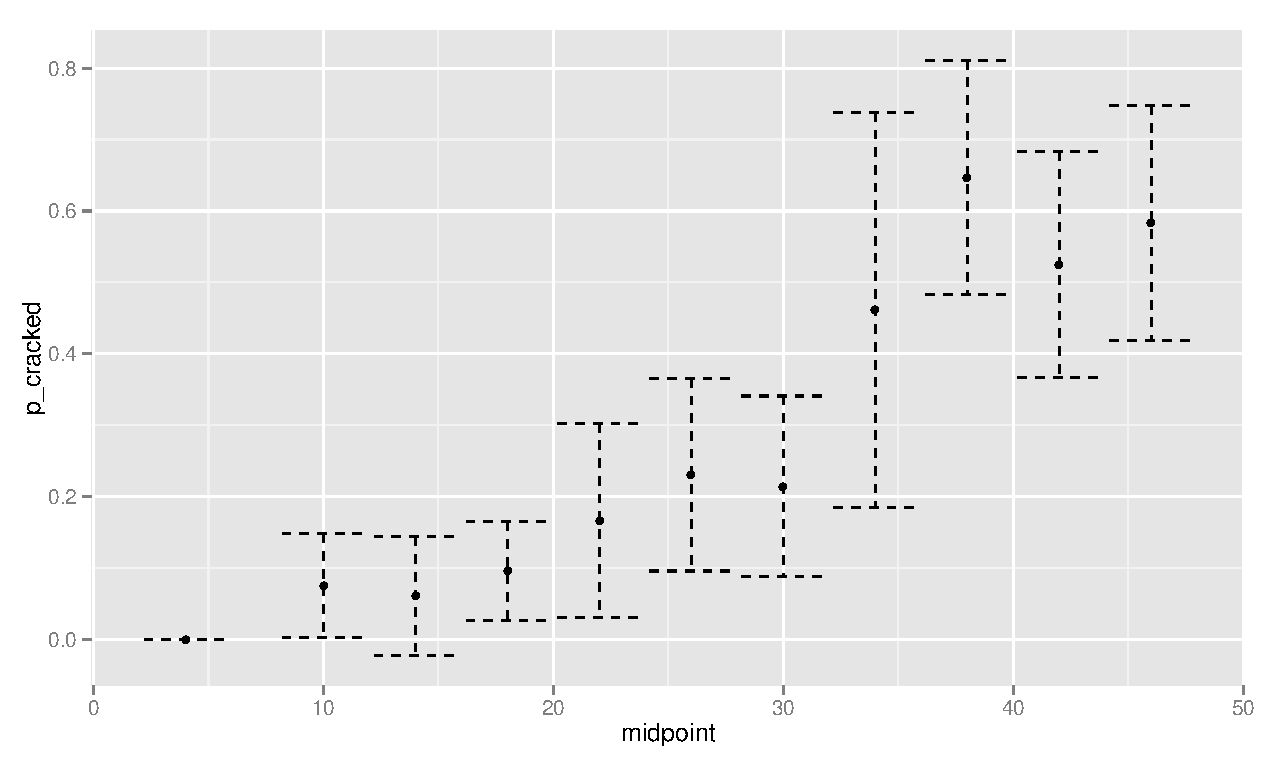
\includegraphics[width=.8\textwidth]{cis}
  \caption{Estimated proportion of failure for turbine wheels and 95\% credible intervals.}
  \end{figure}
  
    \item
    To be able to address objective 1 with the data given, we would need to assume that the failure times are independent and identically distributed. Objective 2 requires that the distribution of failure times will remain the same in the future. Objective 3 would almost certainly be made easier by assuming the unknown distribution belongs to a known parametric family of distributions.
  \end{enumerate}
  \item[1.12]
Graphical methods are useful for identifying special features of the data such as outliers, checking model assumptions and interpreting and communicating results and related uncertainties. 
\end{enumerate}

\end{document}
